
% ---
% Evidência no mundo real
% ---
\chapter{Evidências dos comportamentos seguir ou evitar a multidão }
\label{cap:evidencias}
% ---


	%%% PT-BR version
	A seguir,  visamos identificar na Internet comportamentos que se assemelhem a padrões do tipo   \textit{seguir} ou \textit{evitar} a multidão.
Para tal,	usamos dados reportados em \cite{wang2017characterizing} sobre a aplicação de \emph{patches} por parte dos usuários.    
	De acordo com \cite{wang2017characterizing}, em uma análise de mais de 64 mil amostras de dispositivos  de sistemas de controle industrial, menos de 30\% desses sistemas são atualizados para versões imunes a ataques, dentro de um prazo de 60 dias desde a descoberta da vulnerabilidade.   
	
		
%%% PT-BR version
	\section{Seleção dos dados}
	Adotamos os seguintes critérios para selecionar os sistemas cujos dados são  relevantes para nossas análises: $1)$ selecionamos sistemas que possuem pelo menos duas versões amostradas; $2)$ dado que os sistemas podem ter várias versões, para cada sistema escolhemos as versões mais populares, ou seja, as que estavam presentes em mais dispositivos durante o  histórico de medições; $3)$  excluímos os sistemas que não tiveram ao menos dez dispositivos ativos em uma única medição em qualquer uma das versões mais populares; $4)$ para facilitar e padronizar a caracterização dos sistemas selecionados, numeramos sequencialmente o número das versões, de modo que os valores menores são os mais antigos e valores maiores correspondem aos mais modernos.
	
	\section{Caracterizando o comportamento} Os típicos comportamentos de \textit{seguir} ou \textit{evitar} a multidão foram caracterizados conforme a adoção de versões mais modernas ou mais antigas. O comportamento de \textit{seguir} (resp., \textit{evitar}) a multidão ocorre quando o pico de usuários da versão mais moderna (resp., mais antiga)  \textbf{ocorre após} do pico de usuários da versão mais antiga (resp., mais moderna), mostrando que há um típico comportamento para atualizar (resp., ignorar) as versões mais recentes do sistema, que se propaga pela população.

	
	A Tabela~\ref{tab:shodam} apresenta o resultado da observação do comportamento de \textit{seguir} a multidão (S), \textit{evitar} a multidão (N) e um comportamento indefinido (I), onde não podemos caracterizar nenhum comportamento típico. As duas primeiras colunas se referem respectivamente ao índice da versão mais popular (1\textordmasculine pop) e ao dia no  qual ocorreu a  medição com  maior número de sistemas utilizando a respectiva versão (topo 1\textordmasculine) \footnote{Os dias são medidos com relação à data da primeira coleta.} e as duas próximas colunas referem-se a segunda versão mais popular. A coluna intitulada S/E/I  indica o comportamento típico da população. Para fazer a  classificação do comportamento, definimos  o índice $\iota$=(topo 1\textordmasculine - topo 2\textordmasculine) / (topo 1\textordmasculine + topo 2\textordmasculine).   O caso  $\iota > 0,01$ (resp., $\iota < -0.01$) corresponde ao comportamento de \textit{seguir} (resp., \emph{evitar})  a multidão.   Valores entre $-0,01$ e $0,01$ são  associados a comportamentos indefinidos.
	

	\begin{table}[!htb]
	    \setlength\tabcolsep{1.5pt}
		\centering
		
		\begin{tabular}{|c|c|c|c|c|l|}
			\hline
			\hspace*{-0.15cm} 1\textordmasculine pop 	 & \hspace*{-0.15cm} topo 1\textordmasculine 	 & \hspace*{-0.15cm} 2\textordmasculine pop 	 & \hspace*{-0.15cm} topo 2\textordmasculine 	 & \hspace*{-0.15cm}S/E/I& \hspace*{-0.15cm} Nome do sistema (arquivo) \\
			\hline
			\hspace*{-0.15cm} 11	& \hspace*{-0.15cm} 847	& \hspace*{-0.15cm} 6	& \hspace*{-0.15cm} 268	& \hspace*{-0.15cm} S	& \hspace*{-0.15cm} Allegro RomPager	 \\
			\hspace*{-0.15cm} 2	& \hspace*{-0.15cm} 857	& \hspace*{-0.15cm} 1	& \hspace*{-0.15cm} 854	& \hspace*{-0.15cm} I	& \hspace*{-0.15cm} AMX NetLinx A	 \\
			\hspace*{-0.15cm} 35	& \hspace*{-0.15cm} 833	& \hspace*{-0.15cm} 23	& \hspace*{-0.15cm} 850	& \hspace*{-0.15cm} E	& \hspace*{-0.15cm} Apache httpd	 \\
			\hspace*{-0.15cm} 25	& \hspace*{-0.15cm} 450	& \hspace*{-0.15cm} 21	& \hspace*{-0.15cm} 191	& \hspace*{-0.15cm} S	& \hspace*{-0.15cm} AVM FRITZ!Box Fon WLAN 7170 SIP	 \\
			\hspace*{-0.15cm} 5	& \hspace*{-0.15cm} 831	& \hspace*{-0.15cm} 2	& \hspace*{-0.15cm} 847	& \hspace*{-0.15cm} I	& \hspace*{-0.15cm} Boa HTTPd	 \\
			\hspace*{-0.15cm} 11	& \hspace*{-0.15cm} 156	& \hspace*{-0.15cm} 4	& \hspace*{-0.15cm} 857	& \hspace*{-0.15cm} E	& \hspace*{-0.15cm} Dropbear sshd	 \\
			\hspace*{-0.15cm} 6	& \hspace*{-0.15cm} 757	& \hspace*{-0.15cm} 4	& \hspace*{-0.15cm} 755	& \hspace*{-0.15cm} I	& \hspace*{-0.15cm} Lantronix MSS100 serial interface fingerd	 \\
			\hspace*{-0.15cm} 13	& \hspace*{-0.15cm} 448	& \hspace*{-0.15cm} 8	& \hspace*{-0.15cm} 311	& \hspace*{-0.15cm} S	& \hspace*{-0.15cm} lighttpd	 \\
			\hspace*{-0.15cm} 7	& \hspace*{-0.15cm} 849	& \hspace*{-0.15cm} 5	& \hspace*{-0.15cm} 848	& \hspace*{-0.15cm} I	& \hspace*{-0.15cm} Microsoft IIS httpd	 \\
			\hspace*{-0.15cm} 12	& \hspace*{-0.15cm} 850	& \hspace*{-0.15cm} 6	& \hspace*{-0.15cm} 833	& \hspace*{-0.15cm} S	& \hspace*{-0.15cm} Microsoft SQL Server	 \\
			\hspace*{-0.15cm} 2	& \hspace*{-0.15cm} 558	& \hspace*{-0.15cm} 1	& \hspace*{-0.15cm} 567	& \hspace*{-0.15cm} I	& \hspace*{-0.15cm} MoxaHttp	 \\
			\hspace*{-0.15cm} 45	& \hspace*{-0.15cm} 852	& \hspace*{-0.15cm} 36	& \hspace*{-0.15cm} 833	& \hspace*{-0.15cm} S	& \hspace*{-0.15cm} MySQL	 \\
			\hspace*{-0.15cm} 36	& \hspace*{-0.15cm} 837	& \hspace*{-0.15cm} 8	& \hspace*{-0.15cm} 848	& \hspace*{-0.15cm} I	& \hspace*{-0.15cm} nginx	 \\
			\hspace*{-0.15cm} 33	& \hspace*{-0.15cm} 852	& \hspace*{-0.15cm} 28	& \hspace*{-0.15cm} 852	& \hspace*{-0.15cm} I	& \hspace*{-0.15cm} OpenSSH	 \\
			\hspace*{-0.15cm} 17	& \hspace*{-0.15cm} 857	& \hspace*{-0.15cm} 6	& \hspace*{-0.15cm} 164	& \hspace*{-0.15cm} S	& \hspace*{-0.15cm} ProFTPD	 \\
			\hspace*{-0.15cm} 7	& \hspace*{-0.15cm} 513	& \hspace*{-0.15cm} 5	& \hspace*{-0.15cm} 521	& \hspace*{-0.15cm} I	& \hspace*{-0.15cm} Schneider BMX NOE 0100	 \\
			\hspace*{-0.15cm} 5	& \hspace*{-0.15cm} 532	& \hspace*{-0.15cm} 2	& \hspace*{-0.15cm} 525	& \hspace*{-0.15cm} I	& \hspace*{-0.15cm} Schneider BMX P34 2020	 \\
			\hspace*{-0.15cm} 8	& \hspace*{-0.15cm} 533	& \hspace*{-0.15cm} 7	& \hspace*{-0.15cm} 533	& \hspace*{-0.15cm} I	& \hspace*{-0.15cm} Schneider Electric SAS TSXETY4103	 \\
			\hspace*{-0.15cm} 8	& \hspace*{-0.15cm} 569	& \hspace*{-0.15cm} 6	& \hspace*{-0.15cm} 572	& \hspace*{-0.15cm} I	& \hspace*{-0.15cm} Siemens BACnet Field Panel	 \\
			\hspace*{-0.15cm} 3	& \hspace*{-0.15cm} 564	& \hspace*{-0.15cm} 1	& \hspace*{-0.15cm} 547	& \hspace*{-0.15cm} S	& \hspace*{-0.15cm} Siemens PXG3	 \\
			\hspace*{-0.15cm} 9	& \hspace*{-0.15cm} 1105	& \hspace*{-0.15cm} 8	& \hspace*{-0.15cm} 1096	& \hspace*{-0.15cm} I	& \hspace*{-0.15cm} Siemens SIMATIC IM151	 \\
			\hspace*{-0.15cm} 5	& \hspace*{-0.15cm} 1119	& \hspace*{-0.15cm} 4	& \hspace*{-0.15cm} 1117	& \hspace*{-0.15cm} I	& \hspace*{-0.15cm} Siemens SIMATIC S7 1200	 \\
			\hspace*{-0.15cm} 39	& \hspace*{-0.15cm} 2097	& \hspace*{-0.15cm} 38	& \hspace*{-0.15cm} 2097	& \hspace*{-0.15cm} I	& \hspace*{-0.15cm} Siemens SIMATIC S7 300	 \\
			\hspace*{-0.15cm} 18	& \hspace*{-0.15cm} 838	& \hspace*{-0.15cm} 1	& \hspace*{-0.15cm} 840	& \hspace*{-0.15cm} I	& \hspace*{-0.15cm} Tridium Niagara httpd	 \\
			\hspace*{-0.15cm} 4	& \hspace*{-0.15cm} 845	& \hspace*{-0.15cm} 3	& \hspace*{-0.15cm} 847	& \hspace*{-0.15cm} I	& \hspace*{-0.15cm} Virata-EmWeb	 \\
			\hspace*{-0.15cm} 5	& \hspace*{-0.15cm} 841	& \hspace*{-0.15cm} 4	& \hspace*{-0.15cm} 839	& \hspace*{-0.15cm} I	& \hspace*{-0.15cm} vxTarget ftpd	 \\
			\hspace*{-0.15cm} 7	& \hspace*{-0.15cm} 858	& \hspace*{-0.15cm} 5	& \hspace*{-0.15cm} 858	& \hspace*{-0.15cm} I	& \hspace*{-0.15cm} VxWorks ftpd	 \\
			\hspace*{-0.15cm} 4	& \hspace*{-0.15cm} 856	& \hspace*{-0.15cm} 3	& \hspace*{-0.15cm} 845	& \hspace*{-0.15cm} I	& \hspace*{-0.15cm} WindWeb	 \\
		\hline 	
		\end{tabular}
		\caption{Comportamento   \textit{seguir} ou \textit{evitar} a multidão, observado em populações de usuários de sistemas reais de controle industrial conectados à Internet. A maioria dos produtos possui comportamento típico de \textit{seguir} a multidão, o que vai ao encontro de \textit{evitar} a multidão, típico de sistemas biológicos.}
		\label{tab:shodam}
	\end{table}	

	A Figura~\ref{fig:shodam_example}  ilustra o número de dispositivos adotando cada uma das versões de um determinado produto, ao longo do tempo, para dois produtos distintos (Allegro RomPage e Dropbear sshd). A população do   {Allegro RomPage} possui  comportamento típico de \emph{seguir} a multidão (a versão mais nova substitui a versão mais antiga).  Já o  Dropbear sshd possui  população com comportamento  compatível com \emph{evitar} a multidão. O número de dispositivos com versão antiga cresce em conjunto com o número de dispositivos adotando a versão mais nova do produto. Este último comportamento deve-se, por exemplo, a novas instalações do produto, que muitas vezes podem vir embarcados com versões antigas do firmware.  Mesmo que o comportamento de \emph{evitar} a multidão não esteja sendo tomado de forma consciente e estratégica, os seus impactos são os mesmos que aqueles observados numa população em que indivíduos param de aplicar uma vacina (contramedida), por considerar que a ameaça é desprezível.  Eventualmente,  a população pode  se ver em face a uma epidemia de um vírus que se pensava erradicado.  


	\begin{figure}[!htb]
	%	\centering
	\hspace{-0.2in}	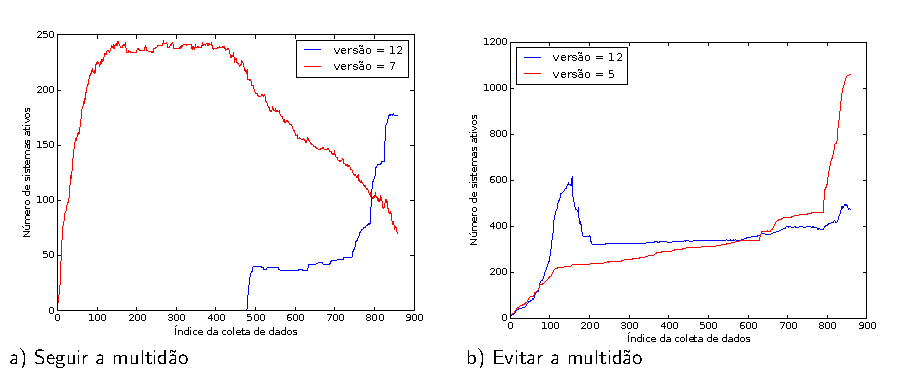
\includegraphics[width=1.0\columnwidth,keepaspectratio=false]{./img/shodam_example.pdf}
		\caption{a) Comportamento de seguir a multidão : sistema Allegro RomPage. b)Comportamento de evitar a multidão: sistema  Dropbear sshd}
		\label{fig:shodam_example}
	\end{figure}

		